\documentclass[hidelinks,12pt]{article}
\usepackage[left=0.25cm,top=1cm,right=0.25cm,bottom=1cm]{geometry}
%\usepackage[landscape]{geometry}
\textwidth = 20cm
\hoffset = -1cm
\usepackage[utf8]{inputenc}
\usepackage[spanish,es-tabla]{babel}
\usepackage[autostyle,spanish=mexican]{csquotes}
\usepackage[tbtags]{amsmath}
\usepackage{nccmath}
\usepackage{amsthm}
\usepackage{amssymb}
\usepackage{mathrsfs}
\usepackage{graphicx}
\usepackage{subfig}
\usepackage{standalone}
\usepackage[outdir=./Imagenes/]{epstopdf}
\usepackage{siunitx}
\usepackage{physics}
\usepackage{color}
\usepackage{float}
\usepackage{hyperref}
\usepackage{multicol}
%\usepackage{milista}
\usepackage{anyfontsize}
\usepackage{anysize}
%\usepackage{enumerate}
\usepackage[shortlabels]{enumitem}
\usepackage{capt-of}
\usepackage{bm}
\usepackage{relsize}
\usepackage{placeins}
\usepackage{empheq}
\usepackage{cancel}
\usepackage{wrapfig}
\usepackage[flushleft]{threeparttable}
\usepackage{makecell}
\usepackage{fancyhdr}
\usepackage{tikz}
\usepackage{bigints}
\usepackage{scalerel}
\usepackage{pgfplots}
\usepackage{pdflscape}
\pgfplotsset{compat=1.16}
\spanishdecimal{.}
\renewcommand{\baselinestretch}{1.5} 
\renewcommand\labelenumii{\theenumi.{\arabic{enumii}})}
\newcommand{\ptilde}[1]{\ensuremath{{#1}^{\prime}}}
\newcommand{\stilde}[1]{\ensuremath{{#1}^{\prime \prime}}}
\newcommand{\ttilde}[1]{\ensuremath{{#1}^{\prime \prime \prime}}}
\newcommand{\ntilde}[2]{\ensuremath{{#1}^{(#2)}}}

\newtheorem{defi}{{\it Definición}}[section]
\newtheorem{teo}{{\it Teorema}}[section]
\newtheorem{ejemplo}{{\it Ejemplo}}[section]
\newtheorem{propiedad}{{\it Propiedad}}[section]
\newtheorem{lema}{{\it Lema}}[section]
\newtheorem{cor}{Corolario}
\newtheorem{ejer}{Ejercicio}[section]

\newlist{milista}{enumerate}{2}
\setlist[milista,1]{label=\arabic*)}
\setlist[milista,2]{label=\arabic{milistai}.\arabic*)}
\newlength{\depthofsumsign}
\setlength{\depthofsumsign}{\depthof{$\sum$}}
\newcommand{\nsum}[1][1.4]{% only for \displaystyle
    \mathop{%
        \raisebox
            {-#1\depthofsumsign+1\depthofsumsign}
            {\scalebox
                {#1}
                {$\displaystyle\sum$}%
            }
    }
}
\def\scaleint#1{\vcenter{\hbox{\scaleto[3ex]{\displaystyle\int}{#1}}}}
\def\bs{\mkern-12mu}


\title{Clase 2 - Estudiando el sistema coordenado cónico \\[0.3em]  \large{Matemáticas Avanzadas de la Física}\vspace{-3ex}}
\author{M. en C. Gustavo Contreras Mayén}
\date{ }

\begin{document}
\vspace{-4cm}
\maketitle
\fontsize{14}{14}\selectfont
\tableofcontents
\newpage

\section{Construcción de sistemas coordenados.}
\subsection{Introducción.}

Una pregunta importante que planteamos en este momento es: ¿para qué estamos revisando los sistemas coordenados curvilíneos?
\par
Como respuesta presentamos la siguiente: Ante un problema de la física, debemos de seleccionar aquel sistema coordenado que mejor se adapte al problema, \emph{para aprovechar cualquier oportunidad o simetría presente en el mismo}.
\par
Recordemos que se modifica una expresión que modela el fenómeno, tal como una ecuación diferencial parcial. De tal manera que con el cambio de sistema coordenado, la solución completa del problema será más fácil que cuando se resuelve en un sistema cartesiano.
\par
Cuando se menciona que \enquote{es más fácil la solución}, significa que se tendrá una ecuación diferencial parcial (EDP) que puede separarse en ecuaciones diferenciales ordinarias (EDO), frecuentemente en la \enquote{forma estándar} en el nuevo sistema coordenado.
\par
La \emph{técnica de separación de variables}, se verá en el Tema 2 del curso.

\section{Desarrollo de un sistema coordenado.}
\subsection{Coordenadas cónicas \texorpdfstring{$(r, \theta, \lambda)$.}{(r, t, l).}}

A continuación veremos la manera de abordar un sistema coordenado especial, para determinar las superficies constantes, los factores de escala, un diferencial de desplazamiento así como los operadores diferenciales, necesarios para resolver un problema con esta geometría en particular.

\subsection{Reglas de transformación.}

Para el sistema coordenado cónico, tenemos que:
\begin{align*}
q_{1} &= r \hspace{1.5cm} 0 \leq r < \infty \\[0.35em]
q_{2} &= \theta \hspace{1.5cm} b^{2} < \theta < c^{2} \\[0.35em]
q_{3} &= \lambda \hspace{1.5cm} 0 < \lambda < b^{2}
\end{align*}
donde $c^{2} > \theta^{2} > b^{2} > \lambda^{2} > 0$
\par
Las reglas de transformación son:
\begin{align*}
x &= \dfrac{r \, \theta \, \lambda}{b \, c} \\[0.5em]
y &= \dfrac{r}{b} \, \sqrt{\dfrac{(\theta^{2} - b^{2})(\lambda^{2} - b^{2})}{(b^{2} - c^{2})}} \\[0.5em]
z &= \dfrac{r}{c} \, \sqrt{\dfrac{(\theta^{2} - c^{2})(\lambda^{2} - c^{2})}{(c^{2} - b^{2})}}
\end{align*}

\subsection{Superficies coordenadas.}

Para identificar las superficies constantes, elevamos al cuadrado cada lado:
\begin{align*}
x^{2} &= \dfrac{r^{2} \theta^{2} \lambda^{2}}{b^{2} c^{2}} \\[0.5em]
y^{2} &= \dfrac{r^{2}}{b^{2}} \dfrac{(\theta^{2} - b^{2})(\lambda^{2} - b^{2})}{(b^{2} - c^{2})} \\[0.5em]
z^{2} &= \dfrac{r^{2}}{c^{2}} \dfrac{(\theta^{2} - c^{2})(\lambda^{2} - c^{2})}{(c^{2} - b^{2})}
\end{align*}

Sumamos las expresiones al cuadrado:
\begin{align*}
x^{2} + y^{2} + z^{2} &= \dfrac{r^{2} \theta^{2} \lambda^{2}}{b^{2} c^{2}} + \dfrac{r^{2}}{b^{2}} \dfrac{(\theta^{2} - b^{2})(\lambda^{2} - b^{2})}{(b^{2} - c^{2})} + \\[0.5em]
&+ \dfrac{r^{2}}{c^{2}} \dfrac{(\theta^{2} - c^{2})(\lambda^{2} - c^{2})}{(c^{2} - b^{2})} =
\end{align*}

Nos armamos con paciencia para resolver la suma de fracciones, el álgebra debe de llevarse con cuidado. Factorizamos el término $r^{2}$:
\begin{align*}
&= r^{2} \bigg[ \dfrac{\theta^{2} \lambda^{2}}{b^{2} c^{2}} + \dfrac{1}{b^{2}} \dfrac{(\theta^{2} - b^{2})(\lambda^{2} - b^{2})}{(b^{2} - c^{2})} + \dfrac{1}{c^{2}} \dfrac{(\theta^{2} - c^{2})(\lambda^{2} - c^{2})}{(c^{2} - b^{2})} \bigg]
\end{align*}

Nos enfocamos con los siguientes sumandos:
\begin{align*}
\dfrac{(\theta^{2} - b^{2})(\lambda^{2} - b^{2})}{b^{2}(b^{2} - c^{2})} + \dfrac{(\theta^{2} - c^{2})(\lambda^{2} - c^{2})}{c^{2}(c^{2} - b^{2})}
\end{align*}

Haciendo con cuidado el álgebra, desarrollamos cada uno de los términos, entonces para el primero:
\begin{align*}
&{}\dfrac{(\theta^{2} - b^{2})(\lambda^{2} - b^{2})}{b^{2}(b^{2} - c^{2})} = \dfrac{\theta^{2} \lambda^{2} - \theta^2 b^{2} - \lambda^{2} b^{2} + b^{4}}{b^{2}(b^{2} - c^{2})} = \\[0.5em] 
&= \dfrac{\theta^{2} \lambda^{2}}{b^{2}(b^{2} - c^{2})} - \dfrac{\theta^{2}}{(b^{2} - c^{2})} - \dfrac{\lambda^{2}}{(b^{2} - c^{2})} + \dfrac{b^{2}}{(b^{2} - c^{2})}
\end{align*}

Entonces para el segundo término:
\begin{align*}
&\dfrac{(\theta^{2} - c^{2})(\lambda^{2} - c^{2})}{c^{2}(c^{2} - b^{2})} = \dfrac{\theta^{2} \lambda^{2} - \theta^2 c^{2} - \lambda^{2} c^{2} + c^{4}}{c^{2}(c^{2} - b^{2})} = \\[0.5em] 
&= \dfrac{\theta^{2} \lambda^{2}}{c^{2}(c^{2} - b^{2})} - \dfrac{\theta^{2}}{(c^{2} - b^{2})} - \dfrac{\lambda^{2}}{(c^{2} - b^{2})} + \dfrac{c^{2}}{(c^{2} - b^{2})}
\end{align*}

Ordenando y sumando los dos términos, tendremos:
\begin{align*}
&\dfrac{\theta^{2} \lambda^{2}}{b^{2}(b^{2} - c^{2})} + \dfrac{\theta^{2} \lambda^{2}}{c^{2}(c^{2} - b^{2})} - \dfrac{\theta^{2}}{(b^{2} - c^{2})} - \dfrac{\theta^{2}}{(c^{2} - b^{2})} + \\[0.5em] 
&- \dfrac{\lambda^{2}}{(b^{2} - c^{2})} - \dfrac{\lambda^{2}}{(c^{2} - b^{2})} + \dfrac{b^{2}}{(b^{2} - c^{2})} + \dfrac{c^{2}}{(c^{2} - b^{2})}
\end{align*}

Del primer término encontrado, vemos que:
\begin{align*}
&{}\dfrac{\theta^{2} \lambda^{2}}{b^{2}(b^{2} - c^{2})} + \dfrac{\theta^{2} \lambda^{2}}{c^{2}(c^{2} - b^{2})} = \\[0.5em] 
&= \dfrac{\theta^{2} \lambda^{2} c^{2} (c^{2} - b^{2}) + \theta^{2} \lambda^{2} b^{2} (b^{2} - c^{2})}{b^{2} c^{2}(b^{2} - c^{2})(c^{2} - b^{2})} = \\[0.5em] 
&= \dfrac{\theta^{2} \lambda^{2} \big[ c^{2} (c^{2} - b^{2}) + b^{2} (b^{2} - c^{2}) \big]}{b^{2} c^{2}(b^{2} - c^{2})(c^{2} - b^{2})} = \\[0.5em] 
&= \dfrac{\theta^{2} \lambda^{2} (c^{4} - b^{2} c^{2} + b^{4} -b^{2} c^{2})}{-b^{2} c^{2} (b^{2} - c^{2})^{2}} = - \dfrac{\theta^{2} \lambda^{2}}{b^{2} c^{2}} \Cancel[red]{\dfrac{(b^{2} - c^{2})^{2}}{(b^{2} - c^{2})^{2}}} = - \dfrac{\theta^{2} \lambda^{2}}{b^{2} c^{2}}
\end{align*}

Entonces el resultado es:
\begin{align*}
\dfrac{\theta^{2} \lambda^{2}}{b^{2}(b^{2} - c^{2})} + \dfrac{\theta^{2} \lambda^{2}}{c^{2}(c^{2} - b^{2})} = - \dfrac{\theta^{2} \lambda^{2}}{b^{2} c^{2}}
\end{align*}

Quedando pendientes los otros términos de la suma. Es fácil revisar que:
\begin{align*}
- \dfrac{\theta^{2}}{(b^{2} {-} c^{2})} {-} \dfrac{\theta^{2}}{(c^{2} {-} b^{2})} &= + \dfrac{\theta^{2}}{(c^{2} {-} b^{2})} {-} \dfrac{\theta^{2}}{(c^{2} {-} b^{2})} = 0 \\[0.5em] 
- \dfrac{\lambda^{2}}{(b^{2} {-} c^{2})} {-} \dfrac{\lambda^{2}}{(c^{2} {-} b^{2})} &= + \dfrac{\lambda^{2}}{(c^{2} {-} b^{2})} {-} \dfrac{\lambda^{2}}{(c^{2} {-} b^{2})} = 0
\end{align*}

El último término que queda es:
\begin{align*}
\dfrac{b^{2}}{(b^{2} - c^{2})} + \dfrac{c^{2}}{(c^{2} - b^{2})} &=  \dfrac{b^{2}}{(b^{2} - c^{2})} - \dfrac{c^{2}}{(b^{2} - c^{2})} = \\[0.5em] 
&= \Cancel[red]{\dfrac{(b^{2} - c^{2})}{(b^{2} - c^{2})}} = 1
\end{align*}

Hemos llegado entonces a que la suma completa es:
\begin{align*}
x^{2} + y^{2} + z^{2} &=  r^{2} \bigg[ \Cancel[blue]{\dfrac{\theta^{2} \lambda^{2}}{b^{2} c^{2}}} - \Cancel[blue]{\dfrac{\theta^{2} \lambda^{2}}{b^{2} c^{2}}} + 1 \bigg] = \\[0.5em] 
x^{2} + y^{2} + z^{2} &= r^{2}
\end{align*}

Que nos definen una familia de esferas concéntricas de radio $r$, siendo la primera superficie coordenada en este sistema cónico.

\begin{figure}[H]
  \centering
  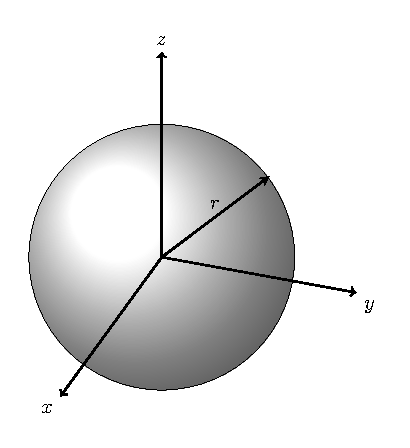
\includegraphics[scale=1]{Imagenes/Sistema_Conico_Superficie_Constante_01.eps}
\end{figure}

\subsection*{Superficie coordenada con \texorpdfstring{$\theta$}{t} constante.}
Al dejar que $\theta$ sea constante, y como $\theta > 0$, podemos revisar lo siguiente:
\begin{align*}
\dfrac{x^{2}}{\theta^{2}} + \dfrac{y^{2}}{\theta^{2} - b^{2}} + \dfrac{z^{2}}{\theta^{2} - c^{2}} = 0
\end{align*}
Que nos define una familia de conos, que es la segunda superficie coordenada.

\subsection*{Superficie coordenada con \texorpdfstring{$\lambda$}{l} constante.}

Ahora hacemos que $\lambda$ sea constante, y como $\lambda > 0$, podemos revisar lo siguiente:
\begin{align*}
\dfrac{x^{2}}{\lambda^{2}} + \dfrac{y^{2}}{\lambda^{2} - b^{2}} + \dfrac{z^{2}}{\lambda^{2} - c^{2}} = 0
\end{align*}

Nos define otra familia de conos, que es la tercera superficie coordenada.

El siguiente paso es intersectar las tres superficies coordenadas:
\begin{figure}[H]
  \centering
  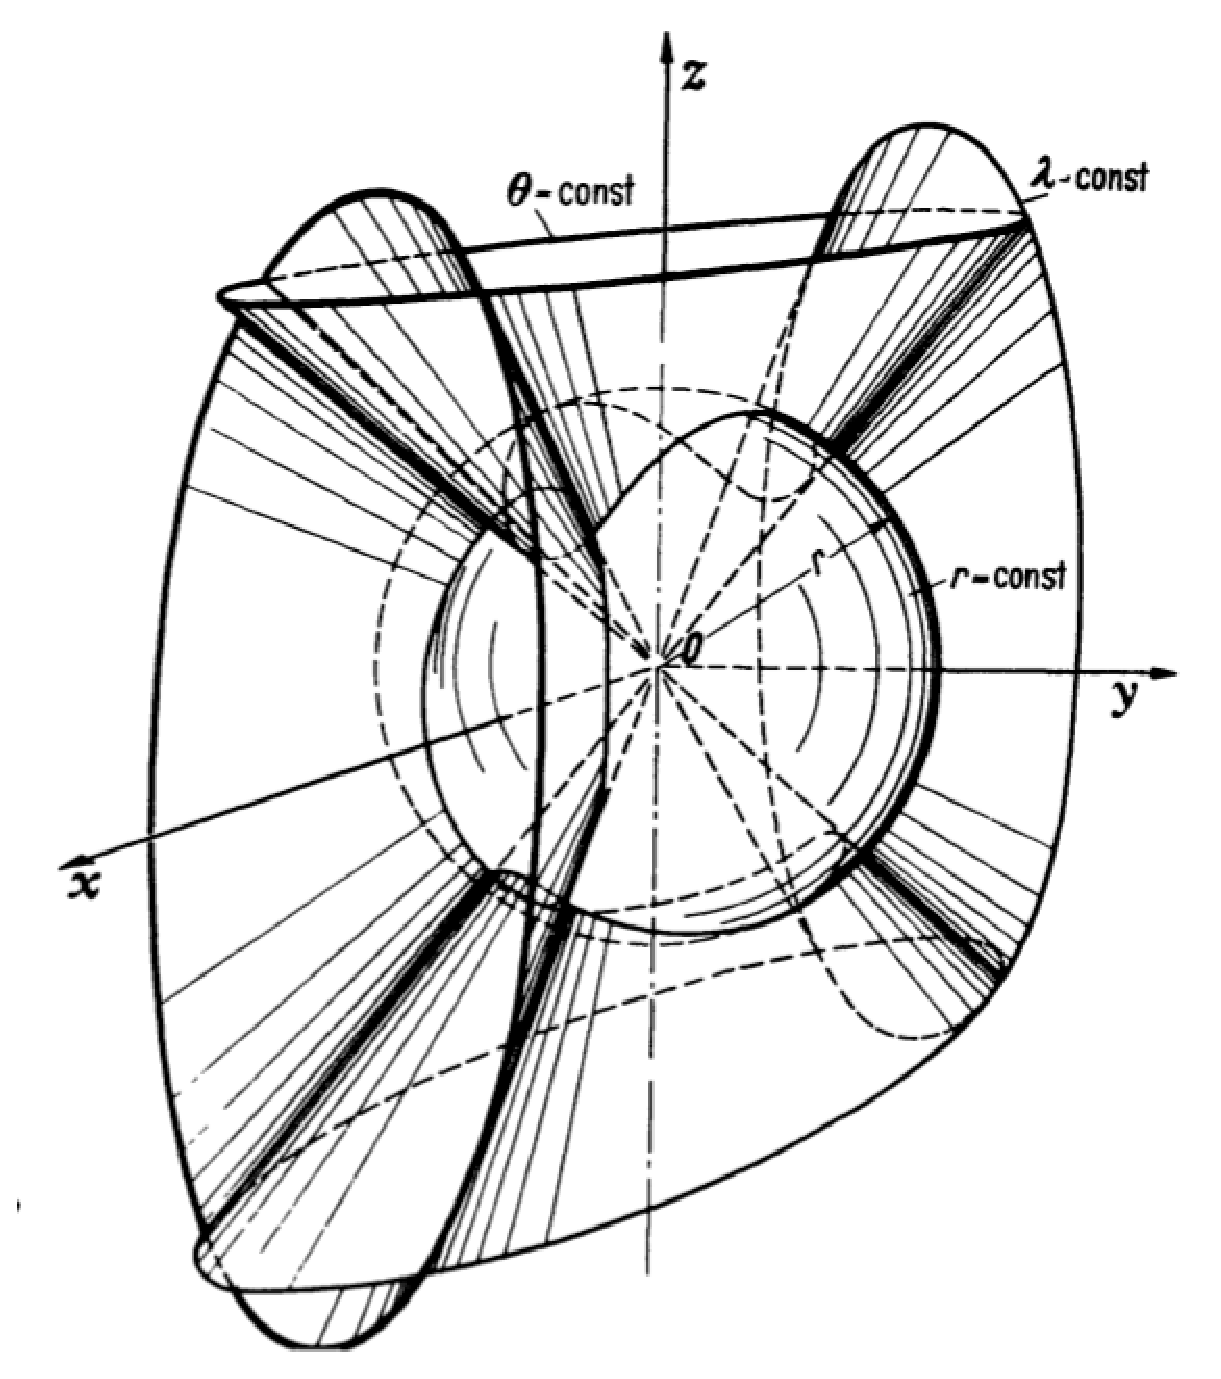
\includegraphics[scale=0.5]{Imagenes/Sistema_Conico.eps}
\end{figure}

\subsection{Factores de escala.}

Para obtener los factores de escala, ocupamos la expresión:
\begin{align*}
h_{i} =  \abs{\dfrac{\dd{\vb{r}}}{u_{i}}} =  \sqrt{\bigg( \pdv{x}{u_{i}} \bigg)^{2} + \bigg( \pdv{y}{u_{i}} \bigg)^{2} + \bigg( \pdv{z}{u_{i}} \bigg)^{2}}
\end{align*}

\subsection*{El factor de escala \texorpdfstring{$h_{r}$}{hr}.}

Para obtener el factor de escala $h_{r}$, debemos de calcular:
\begin{align*}
h_{r} = \sqrt{\bigg( \pdv{x}{r} \bigg)^{2} + \bigg( \pdv{y}{r} \bigg)^{2} + \bigg( \pdv{z}{r} \bigg)^{2}}
\end{align*}

Desarrollamos de manera explícita las derivadas parciales:
\begin{align*}
\pdv{x}{r} &=  \displaystyle \pdv{r} \bigg( \dfrac{r \theta \lambda}{b c} \bigg) =  \dfrac{\theta \lambda}{b c} \hspace{0.3cm} \Rightarrow \hspace{0.3cm} \bigg( \pdv{x}{r} \bigg)^{2} = \dfrac{\theta^{2} \lambda^{2}}{b^{2} c^{2}}
\end{align*}

Para la derivada $\displaystyle \pdv*{y}{r}$, se tiene que:
\begin{align*}
\pdv{y}{r} &=  \pdv{r} \bigg( \dfrac{r}{b} \sqrt{\dfrac{ (\theta^{2} - b^{2}) (\lambda^{2} - b^{2}) }{(b^{2} - c^{2})}} \bigg) = \dfrac{1}{b} \sqrt{\dfrac{ (\theta^{2} - b^{2}) (\lambda^{2} - b^{2}) }{(b^{2} - c^{2})}} \\[0.5em] 
\Rightarrow \hspace{0.3cm} \bigg( \pdv{y}{r} \bigg)^{2} &= \dfrac{1}{b^{2}} \dfrac{ (\theta^{2} - b^{2}) (\lambda^{2} - b^{2})}{(b^{2} - c^{2})}
\end{align*}

Para la derivada $\displaystyle \pdv*{z}{r}$, la expresión a desarrollar es:
\begin{align*}
\pdv{z}{r} &=  \pdv{r} \bigg( \dfrac{r}{c} \sqrt{\dfrac{ (\theta^{2} - c^{2}) (\lambda^{2} - c^{2}) }{(c^{2} - b^{2})}} \bigg) = \dfrac{1}{c} \sqrt{\dfrac{ (\theta^{2} - c^{2}) (\lambda^{2} - c^{2}) }{(c^{2} - b^{2})}} \\[0.5em] 
\Rightarrow \hspace{0.3cm} \bigg( \pdv{z}{r} \bigg)^{2} &= \dfrac{1}{c^{2}} \dfrac{ (\theta^{2} - c^{2}) (\lambda^{2} - c^{2}) }{(c^{2} - b^{2})}
\end{align*}

Hacemos la suma de las derivadas parciales:
\begin{align*}
\bigg( \pdv{x}{r} \bigg)^{2} + \bigg( \pdv{y}{r} \bigg)^{2} + \bigg( \pdv{z}{r} \bigg)^{2} =
\end{align*}

Entonces obtenemos:
\begin{align*}
\dfrac{\theta^{2} \lambda^{2}}{b^{2} c^{2}} + \dfrac{1}{b^{2}} \dfrac{ (\theta^{2} - b^{2}) (\lambda^{2} - b^{2})}{(b^{2} - c^{2})} + \dfrac{1}{c^{2}} \dfrac{ (\theta^{2} - c^{2}) (\lambda^{2} - c^{2}) }{(c^{2} - b^{2})}
\end{align*}

Esta suma es idéntica a la que se encontró al momento de sumar \break \hfill $x^{2} + y^{2} + z^{2}$ (salvo el factor $r^{2}$), por lo que podemos abreviar el trabajo y ocupar el resultado, entonces tenemos que el factor de escala $h_{r}$ es:
\begin{align*}
h_{r} &= \sqrt{\bigg( \pdv{x}{r} \bigg)^{2} + \bigg( \pdv{y}{r} \bigg)^{2} + \bigg( \pdv{z}{r} \bigg)^{2}} = 1
\end{align*}

\subsection*{El factor de escala \texorpdfstring{$h_{\theta}$}{ht}.}

Ocupamos nuevamente la expresión para obtener el factor de escala $h_{\theta}$:
\begin{align*}
h_{\theta} &= \sqrt{\bigg( \pdv{x}{\theta} \bigg)^{2} + \bigg( \pdv{y}{\theta} \bigg)^{2} + \bigg( \pdv{z}{\theta} \bigg)^{2}}
\end{align*}

Recomendamos hacer el cálculo de las derivadas parciales de manera paulatina, para evitar errores.
\par
Comenzamos con la derivada parcial $\pdv*{x}{\theta}$:
\begin{align*}
\pdv{x}{\theta} =  \displaystyle \pdv{\theta} \bigg( \dfrac{r \theta \lambda}{b c} \bigg) =  \dfrac{r \lambda}{b c} \hspace{0.3cm} \Rightarrow \hspace{0.3cm} \bigg( \pdv{x}{\theta} \bigg)^{2} &= \dfrac{r^{2} \lambda^{2}}{b^{2} c^{2}}
\end{align*}

Ahora calcular la derivada parcial $\pdv*{y}{\theta}$:
\begin{align*}
\pdv{y}{\theta} &=  \pdv{\theta} \bigg( \dfrac{r}{b} \sqrt{\dfrac{ (\theta^{2} {-} b^{2}) (\lambda^{2} {-} b^{2}) }{(b^{2} {-} c^{2})}} \bigg) = \dfrac{r \theta (\lambda^{2} {-} b^{2})}{b (b^{2} {-} c^{2}) \bigg[ \dfrac{(\theta^{2} {-} b^{2})(\lambda^{2} {-} b^{2})}{(b^{2} {-} c^{2})} \bigg]^{\frac{1}{2}}} \\[0.5em]
\Rightarrow \hspace{0.1cm} \bigg( \pdv{y}{\theta} \bigg)^{2} &= \dfrac{r^{2} \theta^{2} (\lambda^{2} - b^{2})^{2}}{b^{2} (b^{2} {-} c^{2})^{2} \bigg[ \dfrac{(\theta^{2} {-} b^{2})(\lambda^{2} {-} b^{2})}{(b^{2} {-} c^{2})} \bigg]} = \dfrac{r^{2} \theta^{2} (\lambda^{2} {-} b^{2})}{b^{2} (b^{2} {-} c^{2}) (\theta^{2} {-} b^{2})}
\end{align*}  

Continuamos con la derivada parcial $\pdv*{z}{\theta}$:
\begin{align*}
\pdv{z}{\theta} &=  \pdv{\theta} \bigg( \dfrac{r}{c} \sqrt{\dfrac{(\theta^{2} {-} c^{2})(\lambda^{2} {-} c^{2})}{(c^{2} {-} b^{2})}} \bigg) = \dfrac{r \theta (\lambda^{2} {-} c^{2})}{c (c^{2} {-} b^{2}) \bigg[ \dfrac{(\theta^{2} {-} c^{2})(\lambda^{2} {-} c^{2})}{(c^{2} {-} b^{2})} \bigg]^{\frac{1}{2}}} \\[0.5em]
\Rightarrow \hspace{0.1cm} \bigg( \pdv{z}{\theta} \bigg)^{2} &= \dfrac{r^{2} \theta^{2} (\lambda^{2} {-} c^{2})^{2}}{c^{2} (c^{2} {-} b^{2})^{2} \bigg[ \dfrac{(\theta^{2} {-} c^{2})(\lambda^{2} {-} c^{2})}{(c^{2} {-} b^{2})} \bigg]} = \dfrac{r^{2} \theta^{2} (\lambda^{2} - c^{2})^{2}}{c^{2} (c^{2} - b^{2}) (\theta^{2} - c^{2})}
\end{align*}

Al sumar las tres derivadas parciales, se tiene que:
\begin{align*}
h_{\theta} &= \sqrt{\bigg( \pdv{x}{\theta} \bigg)^{2} + \bigg( \pdv{y}{\theta} \bigg)^{2} + \bigg( \pdv{z}{\theta} \bigg)^{2}} = \\[0.5em] 
&= \dfrac{r^{2} \lambda^{2}}{b^{2} c^{2}} {+} \dfrac{r^{2} \theta^{2} (\lambda^{2} - b^{2})}{b^{2} (b^{2} - c^{2}) (\theta^{2} - b^{2})} {+} \dfrac{r^{2} \theta^{2} (\lambda^{2} - c^{2})^{2}}{c^{2} (c^{2} - b^{2}) (\theta^{2} - c^{2})}
\end{align*}

Luego de un cuidadoso trabajo algebraico, se llega al resultado, es decir, el factor de escala $h_{\theta}$:
\begin{align*}
h_{\theta} = r \sqrt{\dfrac{(\theta^{2} - \lambda^{2})}{(\theta^{2} - b^{2})(c^{2} - \theta^{2})}}
\end{align*}

\subsection*{El factor de escala \texorpdfstring{$h_{\lambda}$}{hl}.}

Siguiendo el mismo procedimiento, el tercer factor de escala para este sistema coordenado cónico es:
\begin{align*}
h_{\lambda} = r \sqrt{\dfrac{(\theta^{2} - \lambda^{2})}{(\lambda^{2} - b^{2})(\lambda^{2} - c^{2})}}
\end{align*}

En las soluciones de los ejercicios a cuenta y del examen, se debe de hacer todo el procedimiento de manera explícita.
\par
Hemos calculado los tres factores de escala:
\begin{align*}
h_{r} &= 1 \\[0.5em]
h_{\theta} &=  r \, \sqrt{\dfrac{(\theta^{2} - \lambda^{2})}{(\theta^{2} - b^{2})(c^{2} - \theta^{2})}} \\[0.5em]
h_{\lambda} &= r \, \sqrt{\dfrac{(\theta^{2} - \lambda^{2})}{(\lambda^{2} - b^{2})(\lambda^{2} - c^{2})}}
\end{align*}


\section{Diferencial de desplazamiento.}
\subsection{Vectores unitarios en el sistema cónico.}

De acuerdo con las notas de trabajo, los vectores unitarios se expresan como:
\begin{align*}
\vu{e}_{i} = \dfrac{1}{h_{i}} \, \pdv{\vb{r}}{u_{i}}
\end{align*}

\subsection{Diferencial de desplazamiento.}

El cuadrado de la distancia entre dos puntos está dado por:
\begin{align*}
\big( \dd{s} \big)^{2} = \big( h_{1} \dd{q_{1}} \big)^{2} + \big( h_{2} \dd{q_{2}} \big)^{2} + \big( h_{3} \dd{q_{3}} \big)^{2}
\end{align*}

Una vez que se cuenta con los factores de escala, podemos expresar el diferencial de desplazamiento en el sistema coordenado cónico:
\begin{align*}
&\big( \dd{s} \big)^{2} = \big( \dd{r} \big)^{2} + r^{2} \big( \theta^{2} {-} \lambda^{2} \big) \bigg[ \dfrac{(\dd{\theta})^{2}}{(\theta^{2} {-} b^{2})(c^{2} {-} \theta^{2})} {+} \dfrac{(\dd{\lambda})^{2}}{(b^{2} {-} \lambda^{2})(c^{2} {-} \lambda^{2})} \bigg]
\end{align*}

Los factores de escala pueden identificarse convenientemente mediante la relación:
\begin{align*}
\dd{s_{i}} = h_{i} \dd{q_{i}}
\end{align*}
para cualquier $\dd{q_{i}}$, conservando las otras $q$ constantes.
\par
Con lo anterior, se pueden desarrollar los elementos de área y volumen:
\begin{align*}
\dd{\sigma_{ij}} &= \dd{s_{i}} \dd{s_{j}} = h_{i} \, h_{j} \dd{q_{i}} \dd{q_{j}} \\[0.5em] 
\dd{\tau} &= \dd{s_{1}} \dd{s_{2}} \dd{s_{3}}= h_{1} \, h_{2} \, h_{3} \dd{q_{1}} \dd{q_{2}} \dd{q_{3}}
\end{align*}
\end{document}